\documentclass[9pt,a4paper]{report}
\usepackage{mwe}
\usepackage{listings}
\usepackage{amsmath}
\usepackage{graphicx}
\usepackage{subfig}
\usepackage{float}
\usepackage{xcolor}
\usepackage{multirow}
\usepackage{hyperref}
\usepackage{fancyhdr}
\usepackage{sectsty}
\usepackage[dvipsnames]{xcolor}
\usepackage{soul}
\usepackage[compact]{titlesec}
\usepackage{float}
\usepackage[left=0.5cm,right=0.5cm,top=0.5cm,bottom=0.5cm]{geometry}
\graphicspath{}

\newcommand*{\nchapter}[1]{%
	\chapter*{#1}%
	\addcontentsline{toc}{chapter}{#1}
	\vspace{-14mm}}
\newcommand*{\nsection}[1]{%
	\section*{#1}%
	\addcontentsline{toc}{section}{#1}}
\newcommand*{\nsubsection}[1]{%
	\subsection*{#1}%
	\addcontentsline{toc}{subsection}{#1}}
\newcommand*{\nsubsubsection}[1]{%
	\subsubsection*{#1}%
	\addcontentsline{toc}{subsubsection}{#1}}

\chaptertitlefont{\large}
\sectionfont{\normalsize}
\fontsize{9}{11}\selectfont
\begin{document}
	\begin{titlepage}
		\centering
		\vspace*{1.5in}
		
\includegraphics[width=0.15\textwidth]{W-Logo_Purple_RGB}\par\vspace{1cm}
		{\LARGE \textsc{University of Washington}\par}
		\vspace{1cm}
		{\Large \textsc{BEE331 Lab 2}\par}
		\vspace{1.5cm}
		{\huge\bfseries \par}
		\vspace{2cm}
		{\Large\itshape 2301991\hspace{55pt}2130474\par}
		{\Large\itshape Jason Truong\hspace{31pt}Henry Haight\par}
		\vfill
		supervised by\par
		Prof.~Joseph \textsc{Decuir}
		\date{2024\\ January}
		\vfill
		% Bottom of the page
		{\large \today\par}
		\vspace*{1.5in}
	\end{titlepage}
	
	\nchapter{MOSFET Bias Circuit}
	\nsection{Design Objective} In this lab we bias a MOSFET for use in both saturation and triode regions. This allows us to maintain a stable DC operating point.
	\nsection{Circuit Design Outline}
	Using our calculated resistors of $38.2k\Omega$ and $95.3k\Omega$ combined with our given resistance values of $500\Omega$ and $200\Omega$ and connecting them to our NMOS transistor in the configureation shown below we can bias our circuit so that the current across the $500\Omega$ and $200\Omega$ ($I_D$) is 10mA. By inputting a voltage of 15V at the leg of the $500\Omega$ resistor we can achive 10mA across the resistors.
	\begin{figure}[hp!] %140, 
		\centering
		\caption{Bias Circuit}
		\subfloat[Bias Circuit Sim]{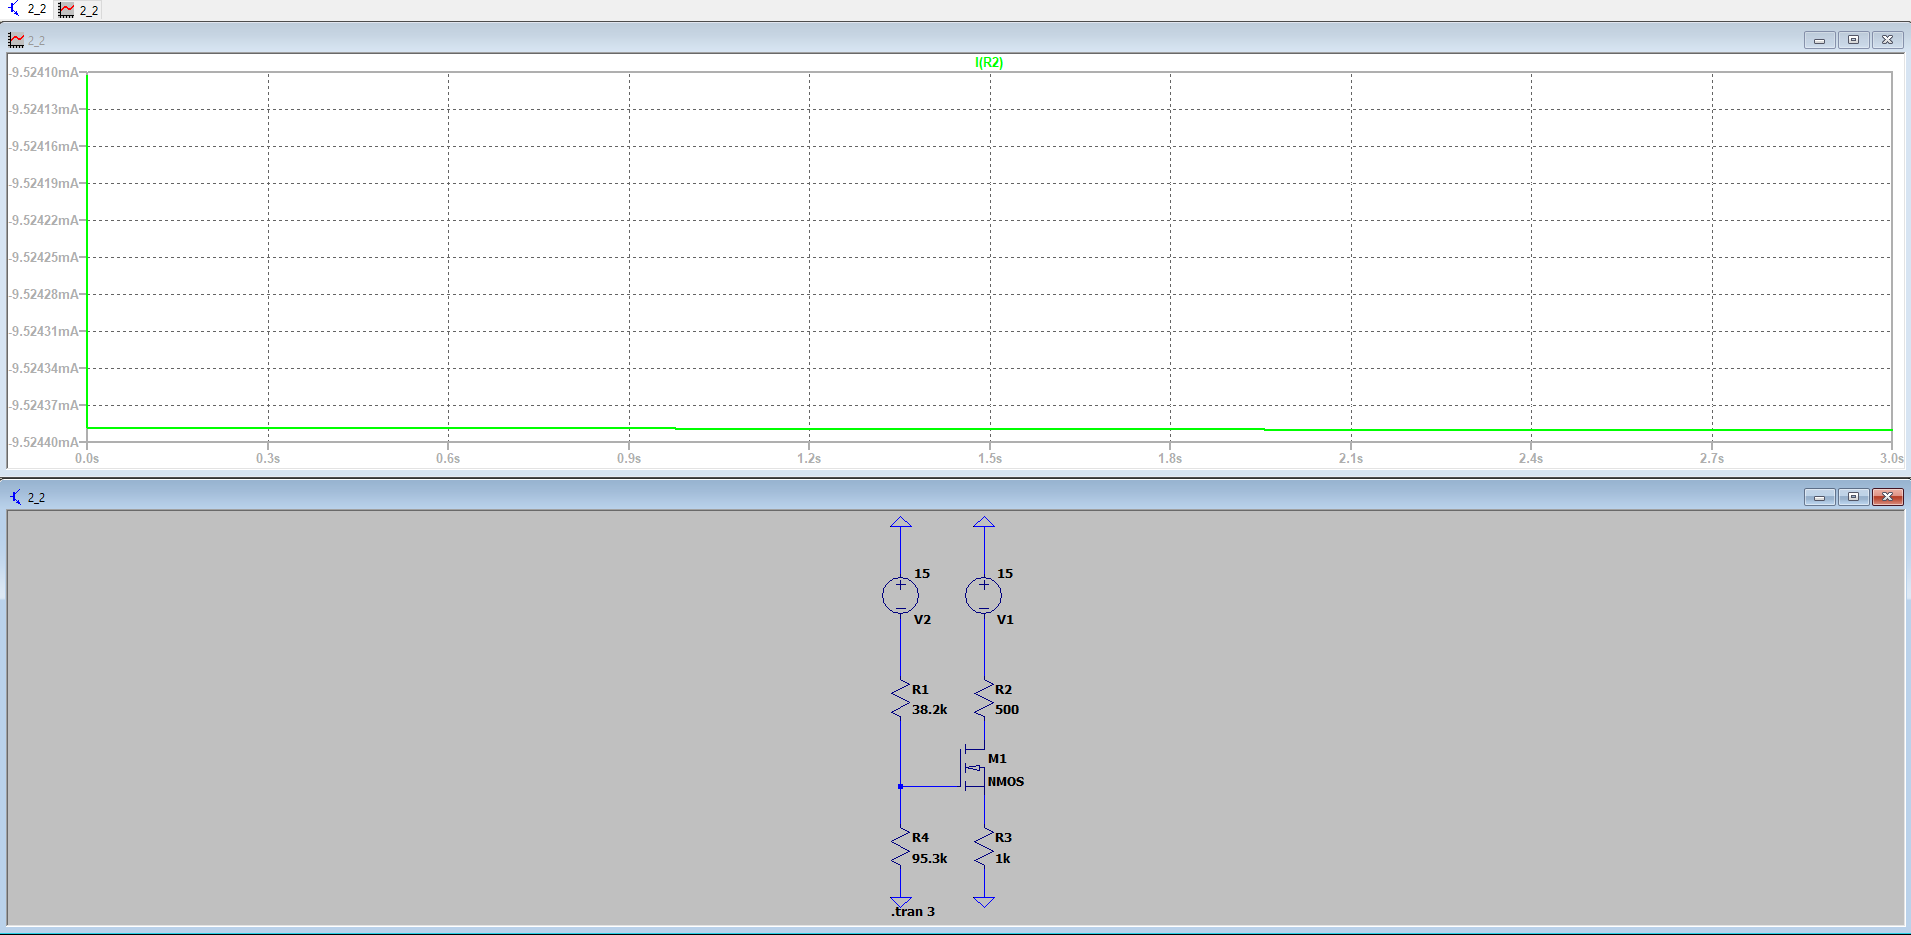
\includegraphics[width=9cm]{SpiceSim}}
	\end{figure}
	\begin{figure}[hp!]
		\ContinuedFloat
		\centering
		\subfloat[\centering Bias Circuit Image]{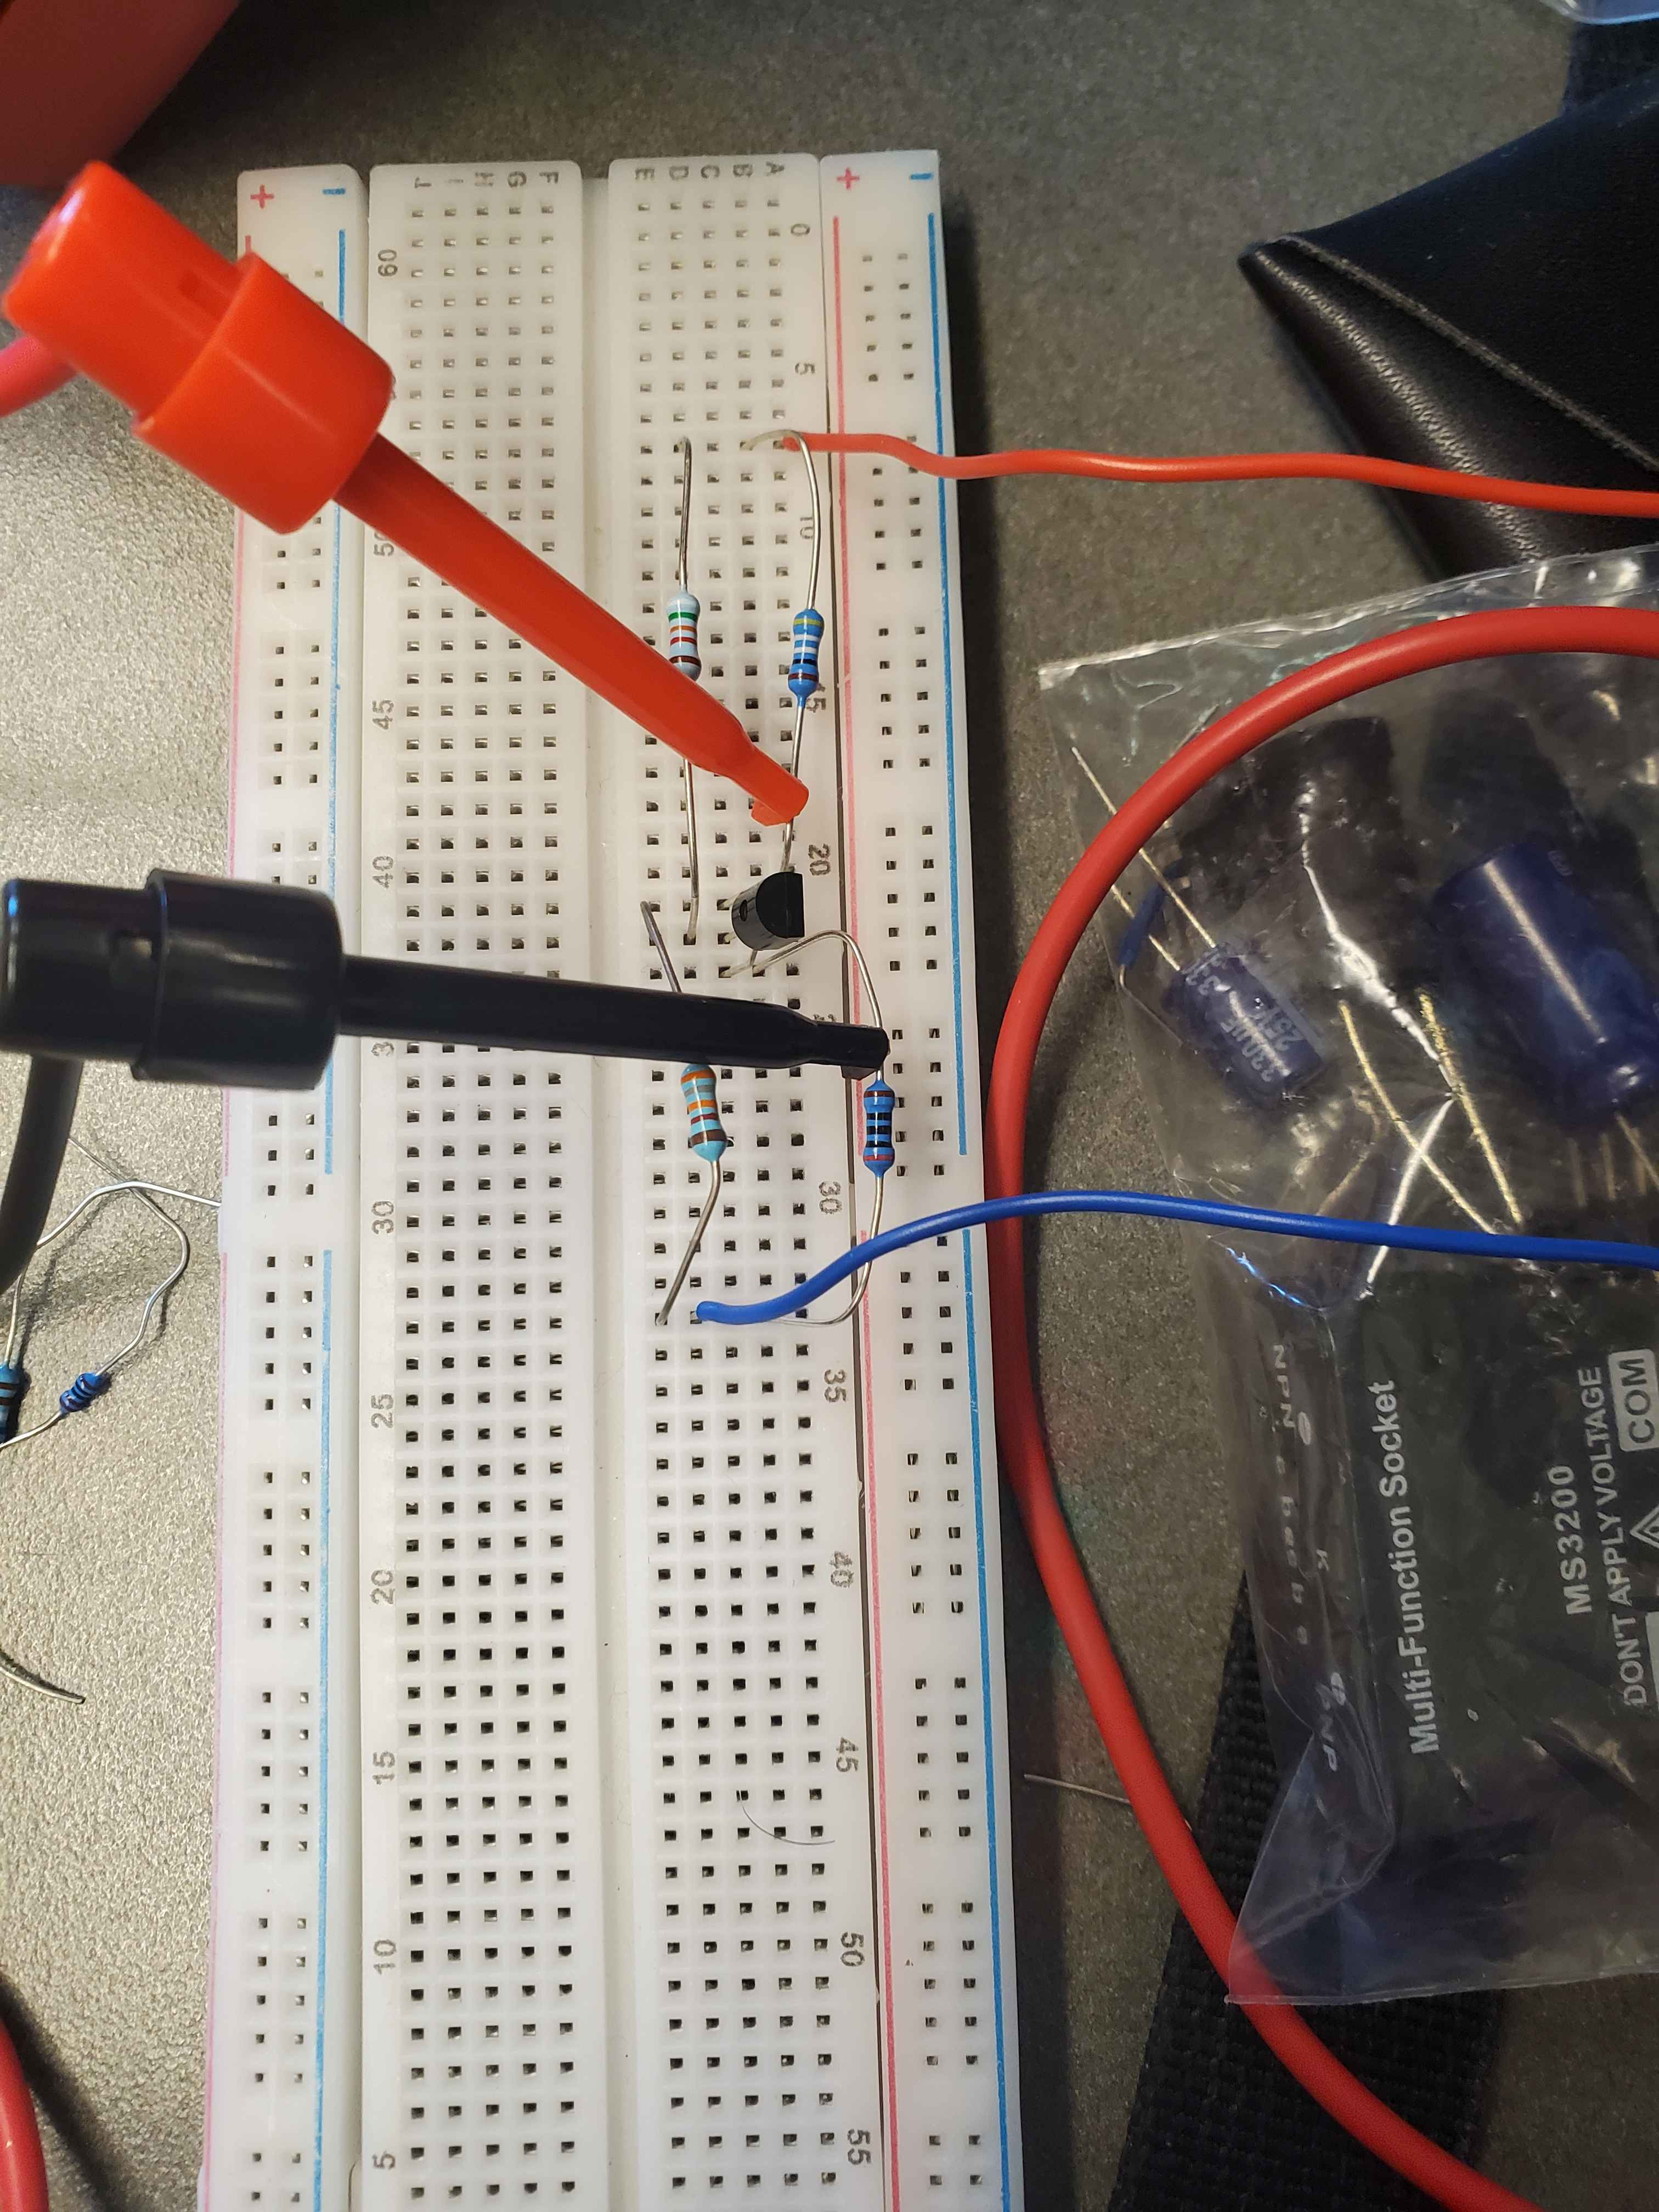
\includegraphics[width=6cm]{CircuitImage}}\hfil
		\subfloat[Bias Circuit Measurement]{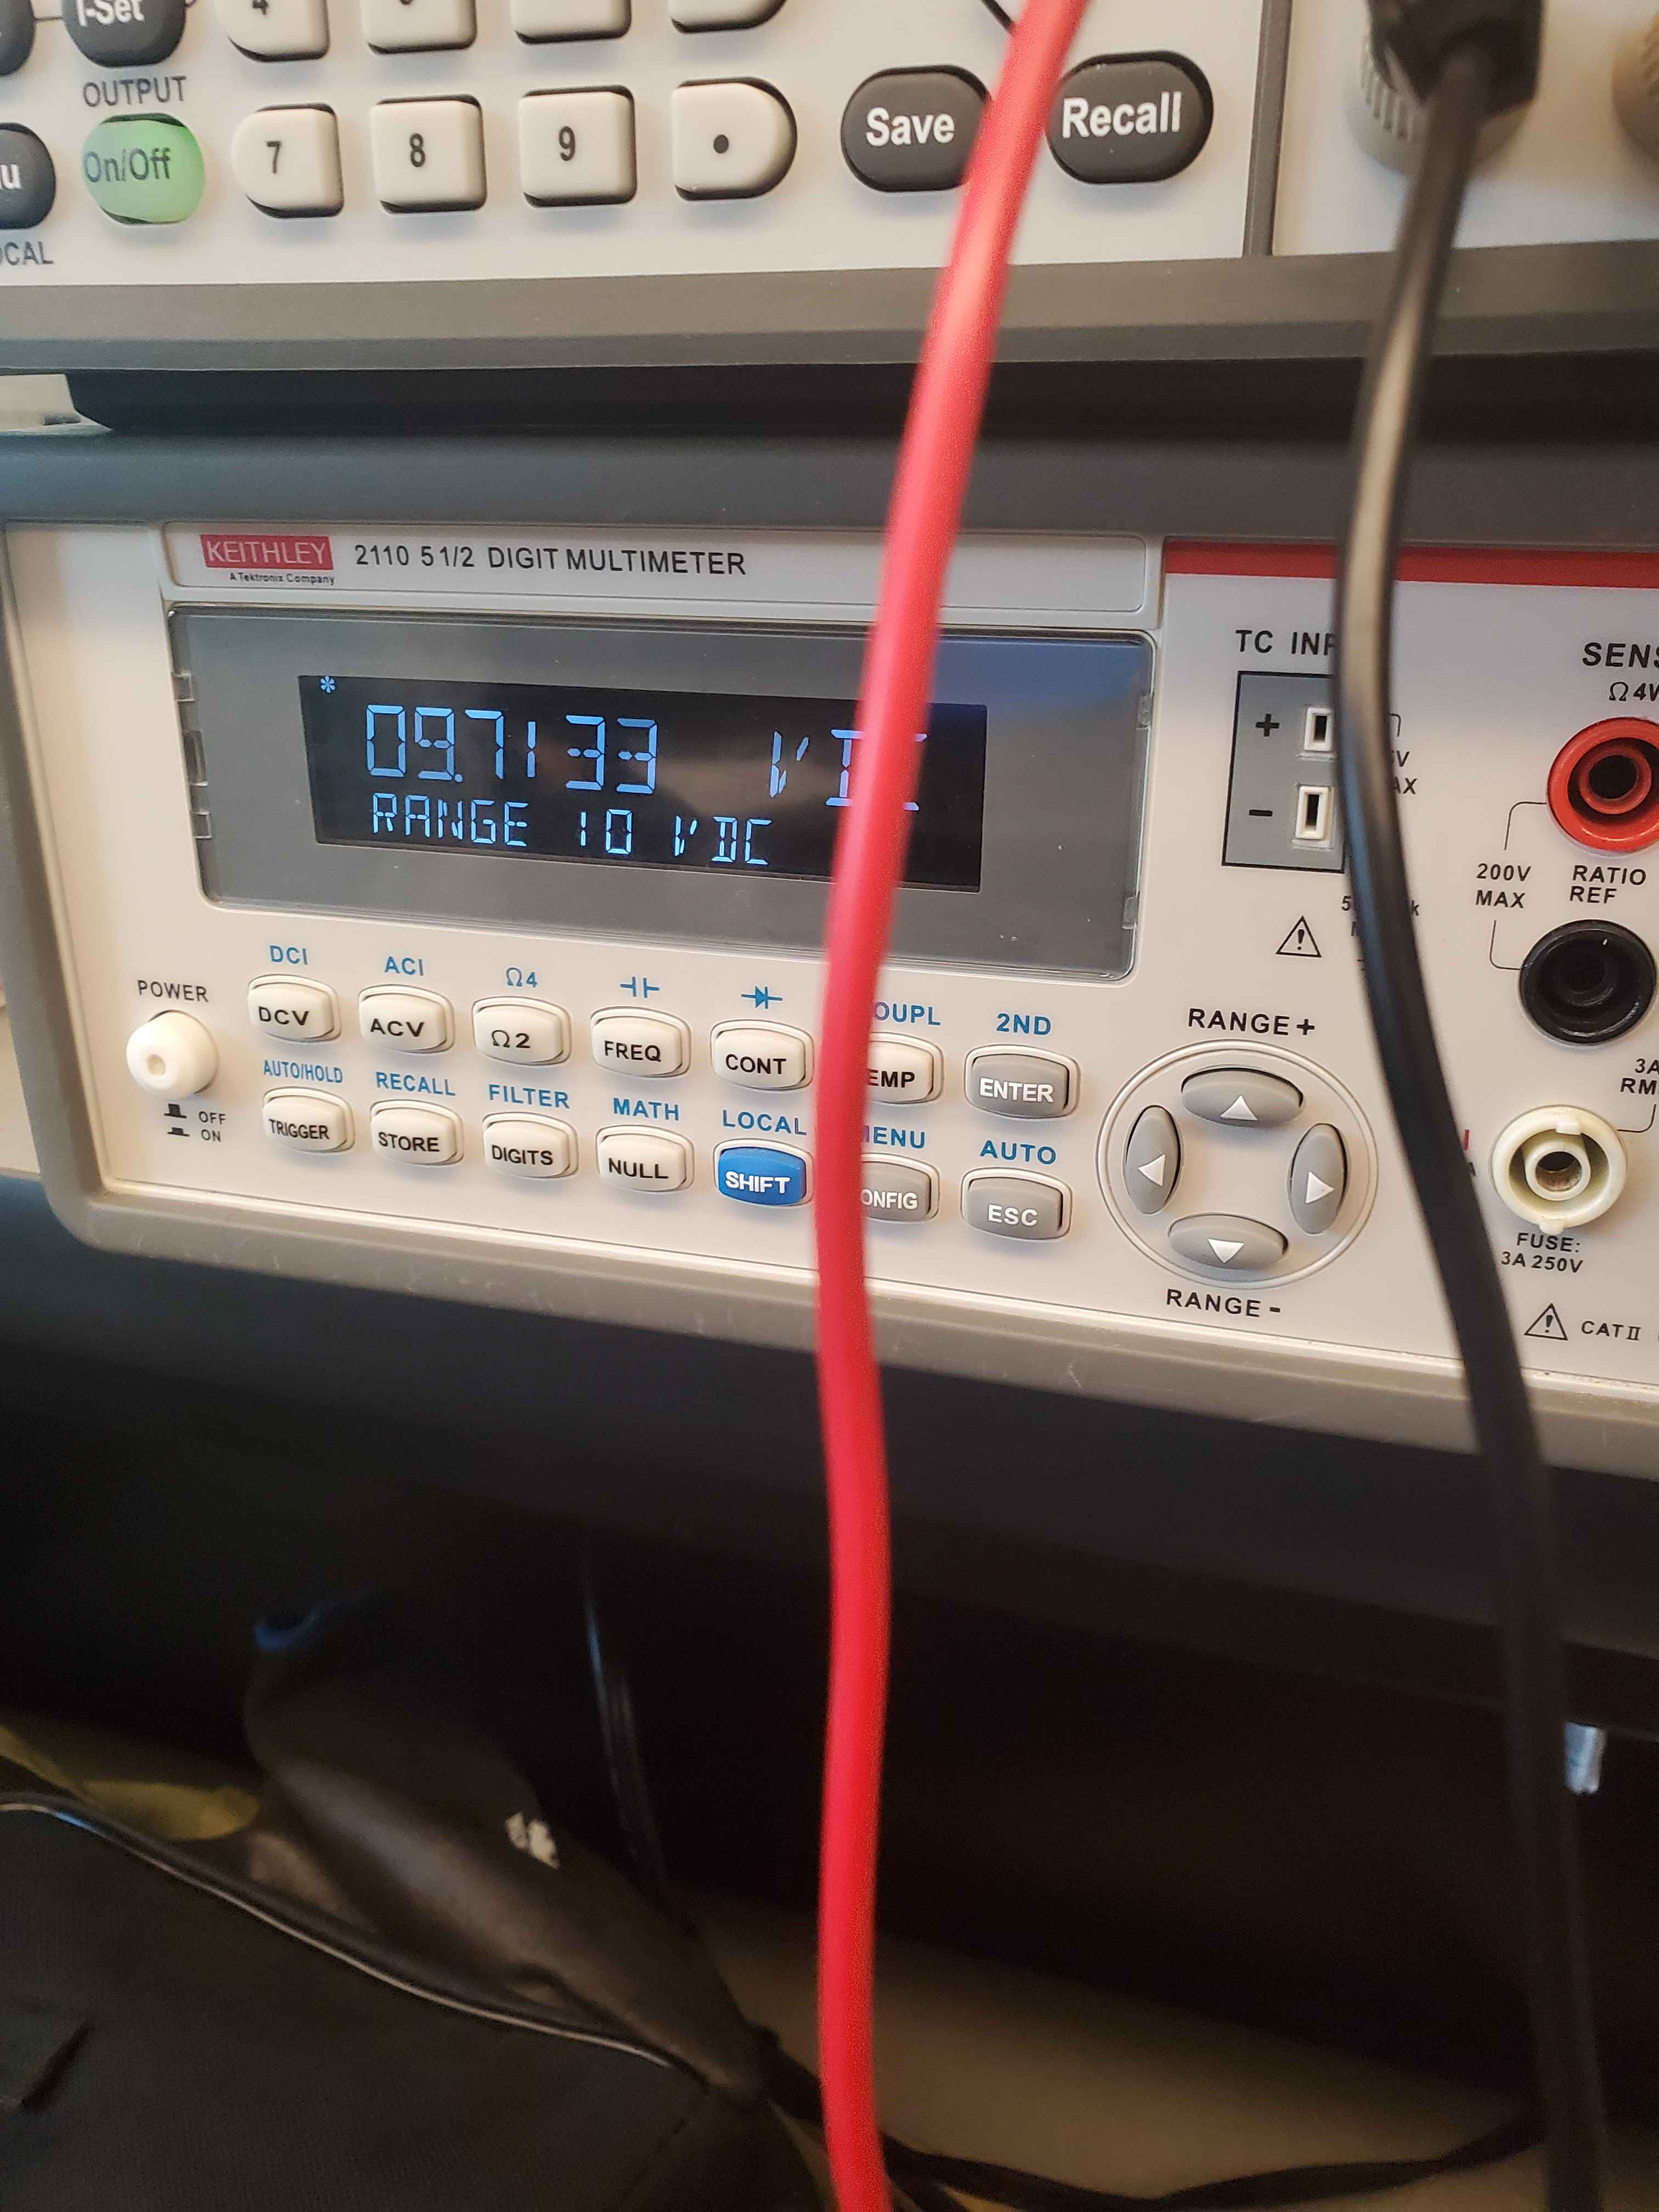
\includegraphics[width=6cm]{VoltageReading}}
	\end{figure}
	\newpage
	\nsection{Measurement and Simulation Results}
	\nsubsection{Analysis}
	\begin{itemize}
		\item \textbf{1. Calculate expected $V_G$, $I_D$ and $V_{DS}$}
		\subitem Using $V_{GS}$ = $V_G$	- $V_S$ and a voltage divider accross the $38.2k\Omega$ and $95.3k\Omega$ resistors we find that $V_G$ = 10.708V.
		\subitem Using the equation $I_D = k_n(V_{GS} - V_T)^2$ we can solve for $I_D$ obtaining $I_D = 10.84mA$ using $k_n = 0.0011$ and $V_T = 1.6$
		\subitem $V_{DS}$ is therefore found using $V_{DS}$ = $V_D$	- $V_S$ where $V_D$ is found using $I_D$, $V_{DD},$ and the $500\Omega$ resistor. This gives us $V_{DS} = 7.411V$
		\item \textbf{2. Compare to simulated results for $V_G$, $I_D$ and $V_{DS}$}
		\subitem The simulated results for $V_G$, $I_D$ and $V_{DS}$ all line up with what we observed during our measurements. The \% difference between the calculated and simulated values are found at a 2\% difference (10.84mA vs 11.04mA).
		\item \textbf{3. Comment on discrepancies}
		\subitem Discrepancies appear from the natural impedance of the NMOS transistor; and the transience of the Gate-Voltage causing a natural and slow rise. As Semiconducting Materials in real life are difficult to keep at a consistent voltage due to them being VERY sensitive and dependent on temperature.
		\subitem 
	\end{itemize}
	
	\nsection{Summary \& Conclusions}
	In this lab, we analysed; characterised; and designed with an NMOSFET transistor for the $I_D$ over both the $V_{GS}$ and $V_{DS}$ region, but also the biasing effects of voltage-dividing over $V_G$
	\end{document}